\chapter{Dataset and Baseline Measures}

\section{Rotterdam Longitudinal Glaucomatous Visual Field Dataset}

The Longitudinal Glaucomatous Visual Field data from Rotterdam Ophthalmic Data Repository \cite{Bryan2013} consists of data from $139$ patients' ($80$ male versus $59$ female) $278$ eyes. A total of $4863$ 24-2 \acl{VF} test results with thresholds and \acp{MD} are available. On average each eye has $17.5$ fields available with mean total follow-up duration of $9.2$ years. $270$ $(97.1\%)$ eyes have at least $14$ fields with a minimum of $7.6$ years of follow-up. The mean and median follow-up interval between tests is $203$ and $189$ days; the standard deviation of follow-up time is $72.3$ days. $346$ $(7.5\%)$ of follow-ups had an interval of more than $270$ days. 

%\begin{figure}[t]
%	\centering
%	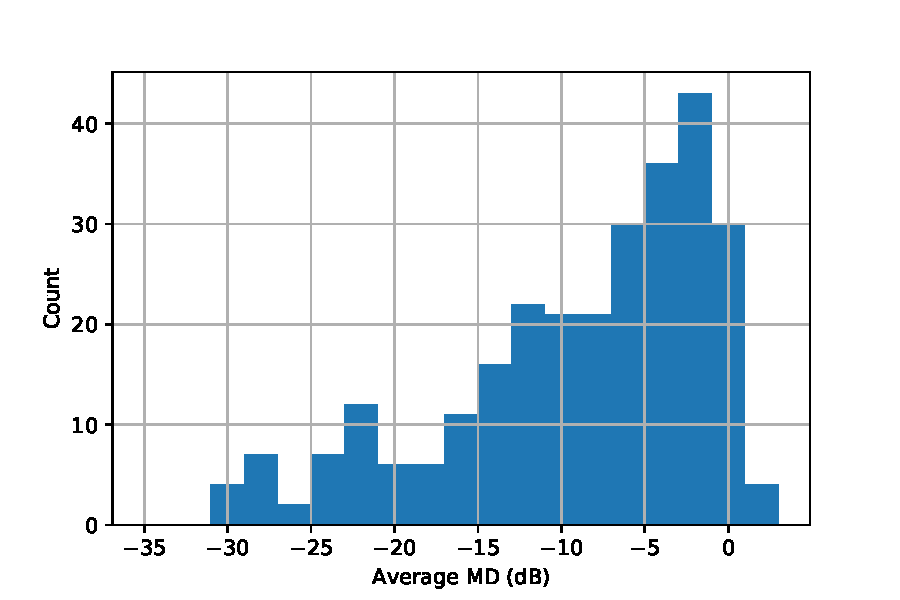
\includegraphics[width=0.6\textwidth]{mean_md_hist}	\caption{Distribution of eyes' average MD values within the Rotterdam dataset ($n=278$)}
%	\label{fig:mean_md_hist}
%\end{figure}

\begin{figure}[p]
	\centering
	\begin{subfigure}[b]{0.49\textwidth}
		\centering
		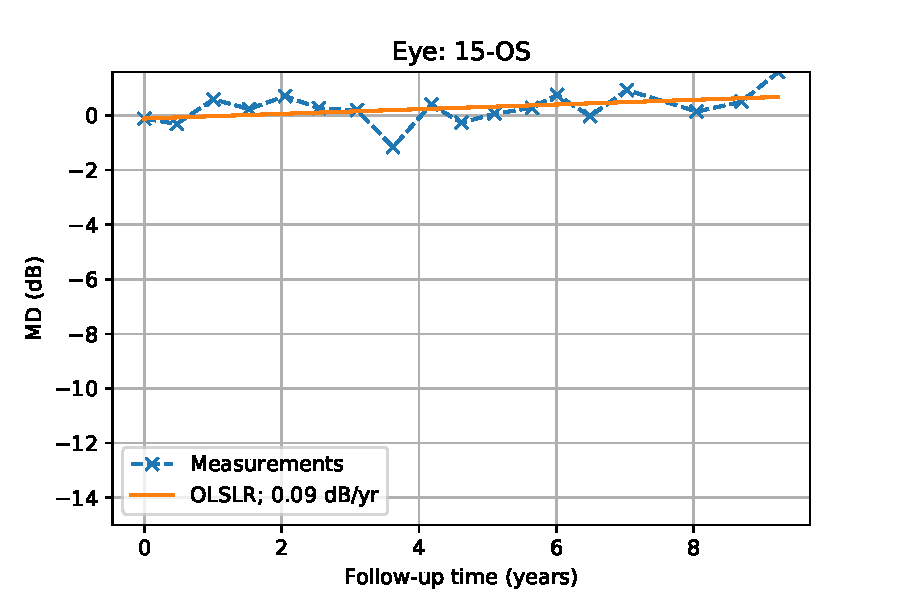
\includegraphics[width=\textwidth]{md_linear/15-OS}
		\caption{A stable healthy eye}
	\end{subfigure}
	\hfill
	\begin{subfigure}[b]{0.49\textwidth}
		\centering
		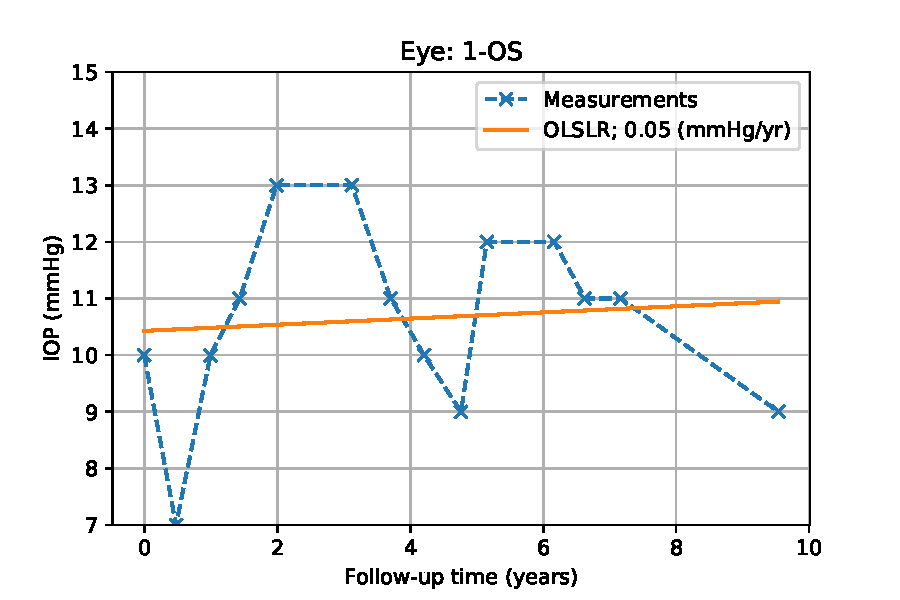
\includegraphics[width=\textwidth]{md_linear/1-OS}
		\caption{A depressed but stable eye}
	\end{subfigure}
	\hfill
	\begin{subfigure}[b]{0.49\textwidth}
		\centering
		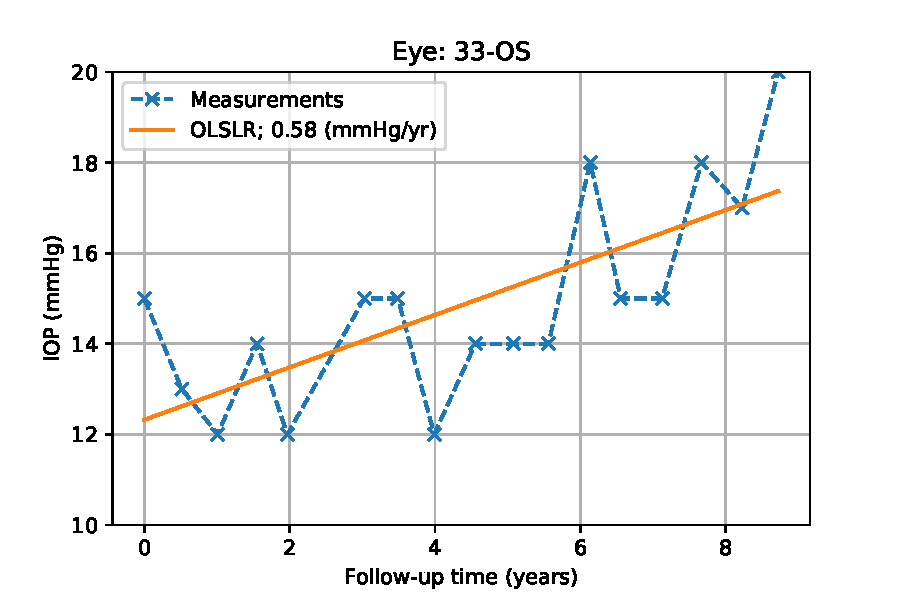
\includegraphics[width=\textwidth]{md_linear/33-OS}
		\caption{A moderately progressing eye}
	\end{subfigure}
	\hfill
	\begin{subfigure}[b]{0.49\textwidth}
		\centering
		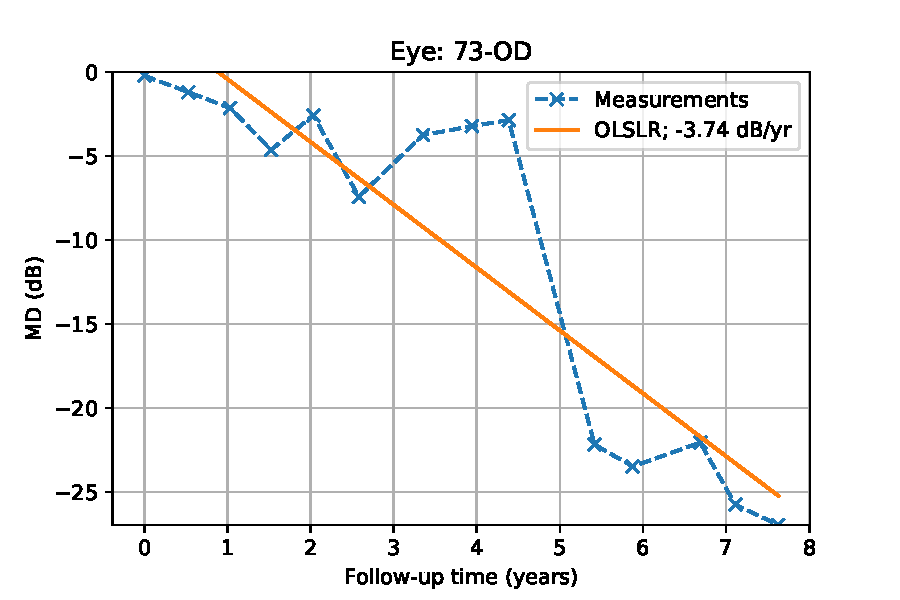
\includegraphics[width=\textwidth]{md_linear/73-OD}
		\caption{A suddenly rapidly progressing eye}
	\end{subfigure}
	\hfill
	\begin{subfigure}[b]{0.49\textwidth}
		\centering
		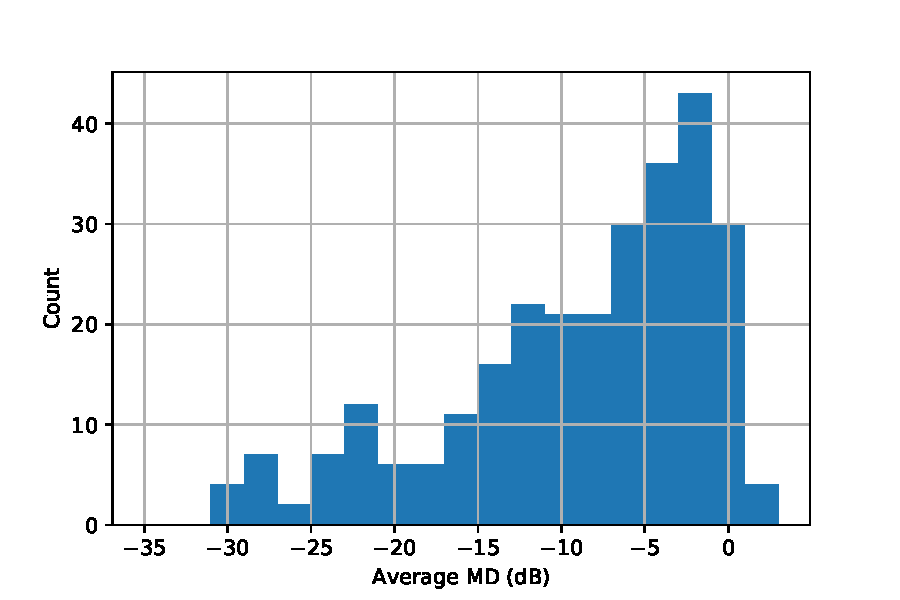
\includegraphics[width=\textwidth]{mean_md_hist}
		\caption{Mean MD}
		\label{fig:mean_md_hist}
	\end{subfigure}
	\hfill
	\begin{subfigure}[b]{0.49\textwidth}
		\centering
		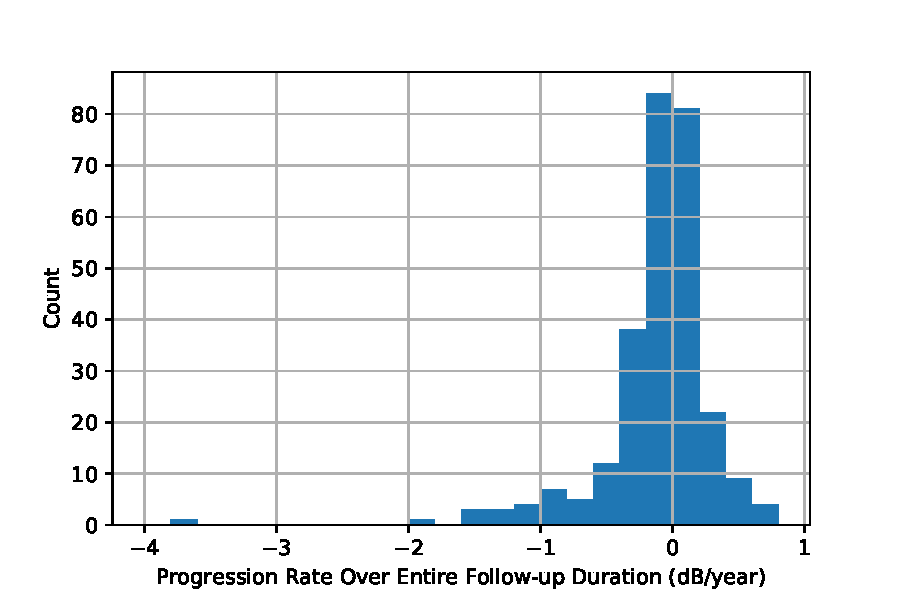
\includegraphics[width=\textwidth]{mdpy_hist}
		\caption{Progression rate $\Delta$MD/yr}
		\label{fig:mdpy_hist}
	\end{subfigure}
	\caption[Overview of the Rotterdam Longitudinal Glaucomatous \acl{VF} Dataset]{Overview of the Rotterdam Longitudinal Glaucomatous \acl{VF} Dataset. (a-d) Select examples of the longitudinal \acl{VF} test results. (e) Distribution of mean MD value over each eye's follow-up duration. A lower mean MD value represents a more depressed eye and likely indicates more severe disease. Not that since perimeters typically have a dynamic range of $0$--$34$ dB, an MD of $-30$ essentially indicates a blind/almost blind eye. (f) Distribution of progression rate of each eye over the follow-up duration as measured by the rate of change of MD. (e-f) shows that a large number of eyes are relatively healthy and most eyes did not progress. This is likely due to either the slowly progressing nature of the glaucoma disease or due to appropriate intervention by clinicians.}
	% 	\label{fig:study_site}
\end{figure}

\subsection{Dataset Characteristics}

To investigate the composition of healthy versus glaucomatous patients the dataset, the characteristic of MD values in the dataset is investigated. In figure \ref{fig:mean_md_hist} the distribution of average MD value calculated from all tests administers on an eye for each of the $278$ eyes is shown. The mean and median of the distribution are $-8.9$ and $-6.8$ dB respectively. The data set contains mostly eyes with mild to moderate reduced MD values ($75\%$ of eyes have average MD $>-13.2$ dB).

To investigate the progression rate in the sample, an \ac{OLSLR} regression line is fit to each eye's MD history. The distribution of the slope (db/year) is shown in figure \ref{fig:mdpy_hist}. 

It is important to note that glaucoma is a very slowly progressing disease. In addition, the data is collected from patients who are undergoing standard treatment. Moreover, both eyes of a glauocma patient are tested, and a patient can often have one glaucomatous eye and another healthy eye. As a result, we see many patients who are healthy (close to $0$ MD) and not progressing (close to $0$ MD/yr).

\section{Performance of Simple Extrapolators}

In this section, using the Rotterdam dataset, we establish a baseline prediction performance using ``naive'' extrapolation methods. 

\subsection{Tasks}

Two prediction tasks evaluated:

\begin{itemize}
	\item \ac{MD} prediction:
	
	This is the traditional, current clinical routine task of predicting future field index value(s) from current known fields and their summaries. 
	
	\item Point-wise prediction:
	
	In this task, instead of predicting one field index that summarizes each future field, the algorithm will output full future field(s) at all $n$ locations. (For 24-2, $n=52+2$ points). This task is usually not attempted traditionally, but in recent years is a common goal of modern machine learning algorithms in this field.
	
\end{itemize}

Both tasks are evaluated with $3$ and $6$ input (``known'') fields to predict the next future first, second, third, \ldots \acl{VF} results. Having $6$ inputs is similar to the current clinical guidelines \cite{Chauhan2008}. Using only $3$ inputs would be more ideal for earlier detection. 

To fully utilize the the data available, all combinations (``prediction series'') of $3$ or $6$ consecutive fields are used for evaluation. For example, for a patient with fields $1$ to $5$, fields $1$ to $3$ are used to predict $4$ and $5$ and fields $2$ to $4$ are used to predict $5$. Details on the generation of testing dataset is described in \cref{sec:datasetgeneration}.

\begin{figure}[p]
	\centering
	\begin{subfigure}[b]{0.49\textwidth}
		\centering
		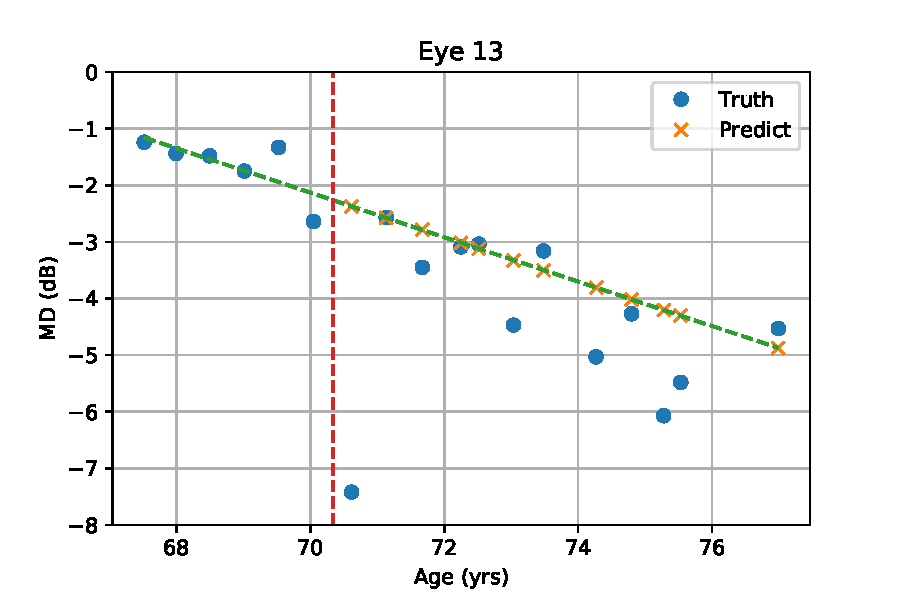
\includegraphics[width=\textwidth]{naive/VFLinearRegressionModel}
		\caption{Linear regression}
	\end{subfigure}
	\hfill
	\begin{subfigure}[b]{0.49\textwidth}
		\centering
		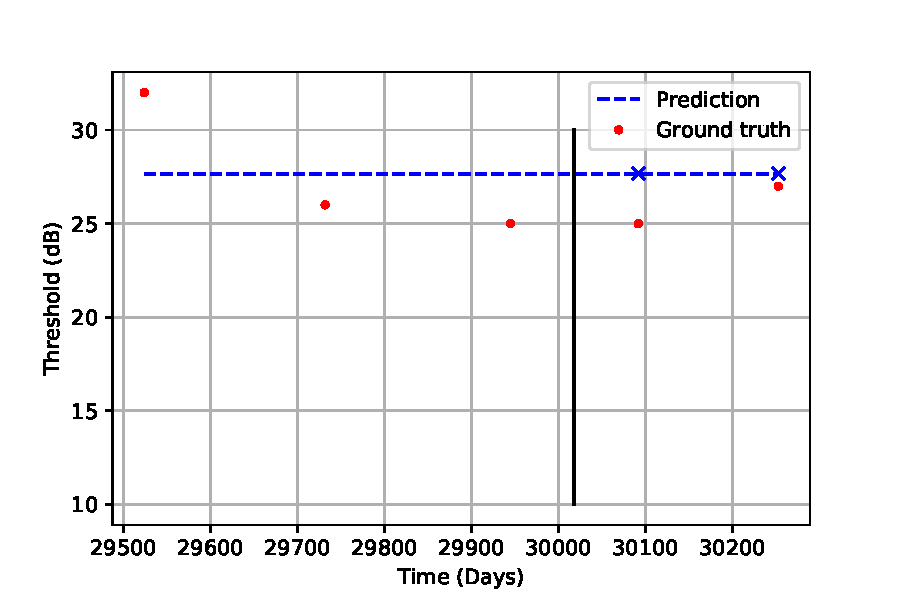
\includegraphics[width=\textwidth]{naive/VFMeanModel}
		\caption{Mean predictor}
	\end{subfigure}
	\hfill
	\begin{subfigure}[b]{0.49\textwidth}
		\centering
		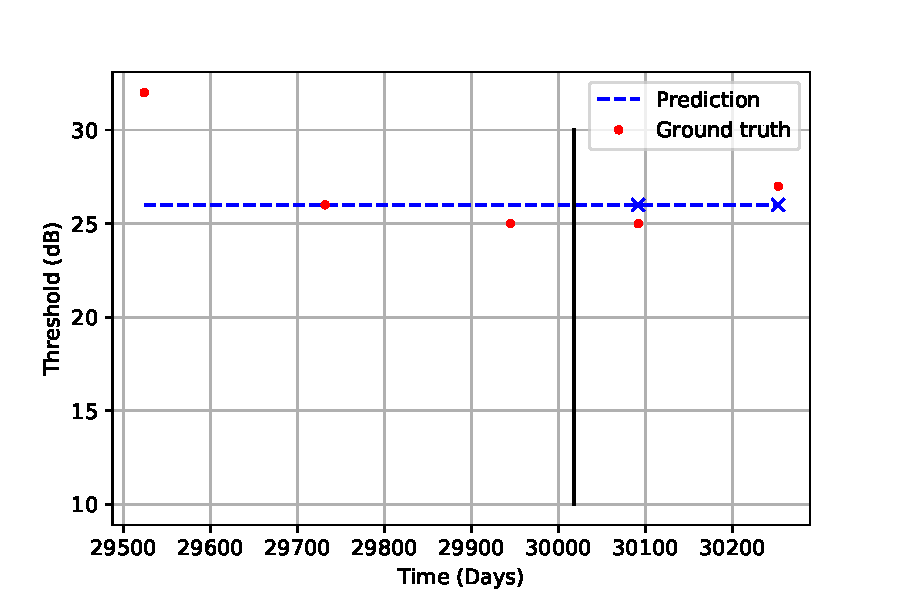
\includegraphics[width=\textwidth]{naive/VFMedianModel}
		\caption{Median predictor}
	\end{subfigure}
	\hfill
	\begin{subfigure}[b]{0.49\textwidth}
		\centering
		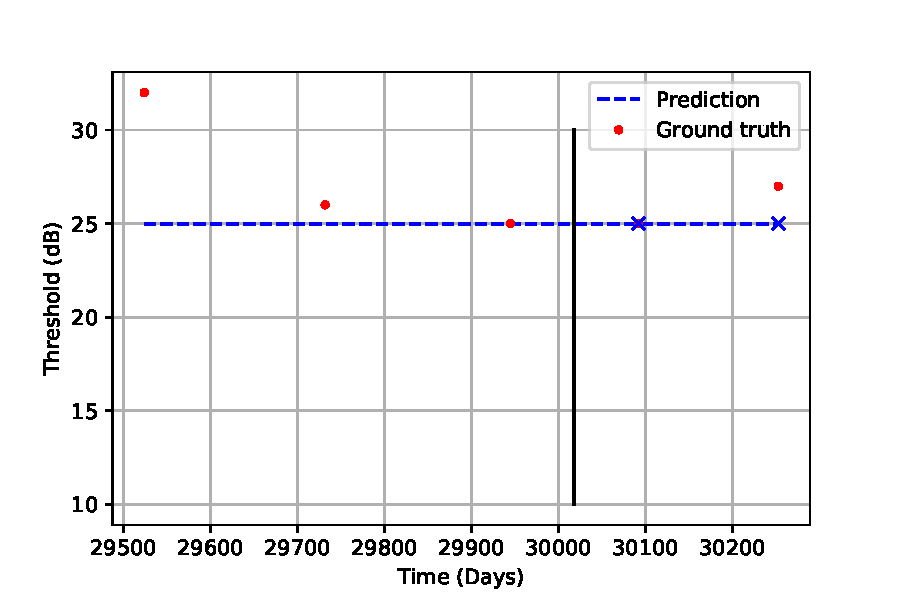
\includegraphics[width=\textwidth]{naive/VFInterpolateModel}
		\caption{Constant extrapolator}
	\end{subfigure}
	\caption{Illustration of the four ``naive'' methods described in \cref{naivemethods}.}
	% 	\label{fig:study_site}
\end{figure}. 


\subsection{Methods} \label{naivemethods}

Inspired by the current widely accepted methods and work by Chen et al. \cite{Chen2014}, the following extrapolation methods are assessed on the dataset:

\begin{itemize}
	\item Linear extrapolation, i.e. \acf{OLSLR}: 
	
	Based on known \ac{MD} and threshold values, predict future corresponding values by linearly fitting and extrapolating on a line that minimizes the sum of squared errors. 
	
	\begin{equation}
		\hat{y}(x)=\mathbf{w}\cdot[1, x]
	\end{equation}
	
	The closed form solution implemented is: 
	
	\begin{equation}
		\mathbf{w}=(X^TX)^{-1}X^Ty
	\end{equation}
	
	where $X\in\mathbb{R}^{m\times 2}$ is the vector of time of $m$ known measurements padded with a column of ones for the bias term. $y\in\mathbb{R}^{m\times n}$ is a matrix of dependent values consisting of rows of measurements (e.g. $n=1$ for \ac{MD} or $n=54$ for 24-2 field thresholds).
	
	\item Repeating mean value:
	
	Predict with a constant value that is the mean of known measurements.
	
	\begin{equation}
		\hat{y}(x)=\textrm{mean}(y)
	\end{equation}
	
	\item Repeating median value:
	
	Predict with a constant value that is the median of known measurements.
	
	\begin{equation}
	\hat{y}(x)=\textrm{median}(y)
	\end{equation}
	
	\item Repeating last value, i.e. nearest neighbor extrapolator:
	
	Extrapolate with the closest value. In the predict task, it means simply taking the last observed value.
	
	\begin{equation}
		\hat{y}(x)=y_m
	\end{equation}
	
\end{itemize}

\subsection{Results for MD Prediction Task}

The \ac{MD} prediction \ac{MAE} for prediction series $i$ is calculated as:

\begin{equation}
\textrm{MAE}({\textrm{MD}_i}) = \left|\widehat{\textrm{MD}_i}-\textrm{MD}_i \right|
\end{equation}

The reported error and standard deviation (STD) is the mean and standard deviation across all $N$ prediction series.

\begin{minipage}{\textwidth}
%\begin{table}[h]
	\captionof{table}{MD prediction performance with 3 input fields}
	\label{tab:md3}
	\resizebox{\textwidth}{!}{%
		\begin{tabular}{rr|llll}
			MD MAE\\$\pm$STD (dB) & N    & Linear      & Mean        & Median      & Extrapolation \\
			\hline
			next 1st        & $3751$ & $1.202\pm1.317$ & $0.991\pm1.110$ & $1.010\pm1.153$ & $1.126\pm1.192$ \\
			next 2nd        & $3751$ & $1.482\pm1.695$ & $1.085\pm1.246$ & $1.094\pm1.282$ & $1.177\pm1.310$ \\
			next 3rd        & $3474$ & $1.788\pm2.096$ & $1.201\pm1.403$ & $1.219\pm1.450$ & $1.275\pm1.402$ \\
			next 4th        & $3197$ & $2.069\pm2.483$ & $1.298\pm1.567$ & $1.319\pm1.618$ & $1.352\pm1.540$ \\
			next 5th        & $2920$ & $2.374\pm2.860$ & $1.414\pm1.725$ & $1.435\pm1.754$ & $1.482\pm1.724$ \\
			next 6th        & $2643$ & $2.651\pm3.281$ & $1.502\pm1.843$ & $1.522\pm1.872$ & $1.551\pm1.835$ \\
			next 7th        & $2366$ & $2.899\pm3.584$ & $1.616\pm1.964$ & $1.635\pm1.996$ & $1.663\pm1.927$ \\
			next 8th        & $2090$ & $3.136\pm3.848$ & $1.697\pm2.051$ & $1.721\pm2.075$ & $1.750\pm2.009$ \\
			next 9th        & $1817$ & $3.406\pm4.127$ & $1.773\pm2.144$ & $1.801\pm2.165$ & $1.843\pm2.083$ \\
			next 10th       & $1546$ & $3.685\pm4.340$ & $1.860\pm2.234$ & $1.878\pm2.254$ & $1.887\pm2.163$ \\
			next 11th       & $1276$ & $3.909\pm4.677$ & $1.961\pm2.292$ & $1.986\pm2.312$ & $2.002\pm2.250$ \\
			next 12th       & $1006$ & $4.088\pm4.861$ & $2.062\pm2.275$ & $2.085\pm2.308$ & $2.070\pm2.254$ \\
			next 13th       & $742$  & $4.329\pm5.212$ & $2.153\pm2.302$ & $2.154\pm2.337$ & $2.205\pm2.316$ \\
			next 14th       & $514$  & $4.861\pm5.613$ & $2.231\pm2.364$ & $2.231\pm2.391$ & $2.287\pm2.391$ \\
			next 15th       & $322$  & $5.357\pm5.978$ & $2.308\pm2.519$ & $2.295\pm2.535$ & $2.315\pm2.501$ \\
			next 16th       & $181$  & $5.639\pm6.306$ & $2.389\pm2.754$ & $2.367\pm2.783$ & $2.484\pm2.702$ \\
			next 17th       & $76$   & $5.916\pm6.828$ & $2.378\pm2.927$ & $2.285\pm2.969$ & $2.428\pm2.910$ \\
			next 18th       & $19$   & $5.699\pm5.530$ & $2.128\pm2.889$ & $2.005\pm2.801$ & $2.229\pm3.175$
		\end{tabular}%
	}
%\end{table}
\end{minipage}


\begin{minipage}{\textwidth}
%\begin{table}[h]
	\captionof{table}{MD prediction performance with 6 input fields}
	\label{tab:md6}
	\resizebox{\textwidth}{!}{%
		\begin{tabular}{rr|llll}
			MD MAE\\$\pm$STD (dB) & N    & Linear      & Mean        & Median      & Extrapolation \\
			\hline
			next 1st        & $2920$ & $1.064\pm1.177$ & $1.070\pm1.289$ & $1.088\pm1.343$ & $1.144\pm1.249$ \\
			next 2nd        & $2920$ & $1.213\pm1.342$ & $1.192\pm1.463$ & $1.208\pm1.525$ & $1.211\pm1.381$ \\
			next 3rd        & $2643$ & $1.352\pm1.504$ & $1.293\pm1.608$ & $1.310\pm1.675$ & $1.283\pm1.459$ \\
			next 4th        & $2366$ & $1.500\pm1.686$ & $1.402\pm1.765$ & $1.418\pm1.810$ & $1.365\pm1.600$ \\
			next 5th        & $2090$ & $1.657\pm1.891$ & $1.502\pm1.863$ & $1.524\pm1.889$ & $1.497\pm1.761$ \\
			next 6th        & $1817$ & $1.792\pm2.002$ & $1.595\pm1.946$ & $1.618\pm1.970$ & $1.573\pm1.850$ \\
			next 7th        & $1546$ & $1.921\pm2.120$ & $1.696\pm2.034$ & $1.714\pm2.068$ & $1.678\pm1.881$ \\
			next 8th        & $1276$ & $2.076\pm2.246$ & $1.793\pm2.100$ & $1.802\pm2.130$ & $1.768\pm1.940$ \\
			next 9th        & $1006$ & $2.218\pm2.364$ & $1.890\pm2.108$ & $1.890\pm2.124$ & $1.867\pm1.977$ \\
			next 10th       & $742$ & $2.367\pm2.613$ & $1.994\pm2.164$ & $1.988\pm2.196$ & $1.949\pm2.055$ \\
			next 11th       & $514$ & $2.533\pm2.845$ & $2.082\pm2.232$ & $2.066\pm2.258$ & $2.035\pm2.189$ \\
			next 12th       & $322$ & $2.745\pm3.159$ & $2.204\pm2.391$ & $2.177\pm2.382$ & $2.154\pm2.311$ \\
			next 13th       & $181$  & $3.048\pm3.719$ & $2.290\pm2.625$ & $2.252\pm2.580$ & $2.356\pm2.640$ \\
			next 14th       & $76$  & $3.312\pm4.085$ & $2.276\pm2.742$ & $2.225\pm2.684$ & $2.377\pm2.812$ \\
			next 15th       & $19$  & $3.445\pm3.240$ & $1.975\pm2.591$ & $1.960\pm2.482$ & $2.301\pm2.494$
		\end{tabular}%
	}
%\end{table}
\end{minipage}

\subsection{Results for Point-Wise \acl{VF} Prediction Task}

In this task, the \ac{MAE} for each predicted field is calculated as:

\begin{equation}
\textrm{MAE}(x_i)=\textrm{mean}(\left\{\left| \hat{x_{i,j}} - x_{i,j} \right|\ \textrm{for}\ j = 1,\ldots,n\right\})
\end{equation}

where $x_i\in\mathbb{R}^{n}$ is a vector representing a visual field test result for eye $i$, and $n$ is the number of points in the test pattern. For 24-2 pattern, $n=54$.

Similar to above, the reported mean and standard deviation is aggregated from all eyes $i\in \left[ 1,N \right]$.

\begin{minipage}{\textwidth}
	%\begin{table}[h]
	\captionof{table}{Point-wise (whole-field) prediction performance with 3 input fields}
	\label{tab:pw3}
	\resizebox{\textwidth}{!}{%
		\begin{tabular}{rr|llll}
			MD MAE\\$\pm$STD (dB) & N    & Linear      & Mean        & Median      & Extrapolation \\
			\hline
			next 1st        & $3751$ & $3.138\pm1.384$ & $2.597\pm1.214$ & $2.598\pm1.252$ & $3.006\pm1.360$ \\
			next 2nd        & $3751$ & $3.597\pm1.593$ & $2.676\pm1.298$ & $2.682\pm1.340$ & $3.069\pm1.436$ \\
			next 3rd        & $3474$ & $4.042\pm1.797$ & $2.770\pm1.398$ & $2.776\pm1.448$ & $3.135\pm1.476$ \\
			next 4th        & $3197$ & $4.458\pm1.990$ & $2.868\pm1.511$ & $2.875\pm1.565$ & $3.214\pm1.567$ \\
			next 5th        & $2920$ & $4.863\pm2.203$ & $2.973\pm1.624$ & $2.982\pm1.668$ & $3.324\pm1.701$ \\
			next 6th        & $2643$ & $5.231\pm2.379$ & $3.058\pm1.704$ & $3.069\pm1.745$ & $3.398\pm1.764$ \\
			next 7th        & $2366$ & $5.581\pm2.500$ & $3.161\pm1.795$ & $3.173\pm1.838$ & $3.494\pm1.827$ \\
			next 8th        & $2090$ & $5.876\pm2.563$ & $3.240\pm1.864$ & $3.258\pm1.912$ & $3.578\pm1.885$ \\
			next 9th        & $1817$ & $6.172\pm2.589$ & $3.329\pm1.945$ & $3.349\pm1.985$ & $3.651\pm1.943$ \\
			next 10th       & $1546$ & $6.447\pm2.695$ & $3.415\pm2.035$ & $3.444\pm2.074$ & $3.722\pm2.011$ \\
			next 11th       & $1276$ & $6.677\pm2.810$ & $3.506\pm2.108$ & $3.533\pm2.154$ & $3.830\pm2.102$ \\
			next 12th       & $1006$ & $6.874\pm2.850$ & $3.593\pm2.134$ & $3.623\pm2.181$ & $3.908\pm2.120$ \\
			next 13th       & $742$  & $7.007\pm2.957$ & $3.694\pm2.212$ & $3.729\pm2.267$ & $4.029\pm2.271$ \\
			next 14th       & $514$  & $7.257\pm3.138$ & $3.743\pm2.277$ & $3.779\pm2.312$ & $4.071\pm2.289$ \\
			next 15th       & $322$  & $7.498\pm3.299$ & $3.902\pm2.483$ & $3.930\pm2.538$ & $4.161\pm2.468$ \\
			next 16th       & $181$  & $7.517\pm3.541$ & $3.972\pm2.541$ & $3.959\pm2.603$ & $4.250\pm2.532$ \\
			next 17th       & $76$   & $7.671\pm3.345$ & $4.208\pm2.913$ & $4.164\pm2.958$ & $4.345\pm2.801$ \\
			next 18th       & $19$   & $7.360\pm3.220$ & $3.656\pm2.187$ & $3.676\pm2.307$ & $3.917\pm2.361$
		\end{tabular}%
	}
	%\end{table}
\end{minipage}


\begin{minipage}{\textwidth}
	%\begin{table}[h]
	\captionof{table}{Point-wise (whole-field) prediction performance with 6 input fields}
	\label{tab:pw6}
	\resizebox{\textwidth}{!}{%
		\begin{tabular}{rr|llll}
			MD MAE\\$\pm$STD (dB) & N    & Linear      & Mean        & Median      & Extrapolation \\
			\hline
			next 1st        & $2920$ & $2.737\pm1.235$ & $2.566\pm1.298$ & $2.533\pm1.350$ & $3.023\pm1.388$ \\
			next 2nd        & $2920$ & $2.940\pm1.347$ & $2.676\pm1.426$ & $2.650\pm1.490$ & $3.105\pm1.484$ \\
			next 3rd        & $2643$ & $3.127\pm1.431$ & $2.769\pm1.527$ & $2.746\pm1.594$ & $3.150\pm1.511$ \\
			next 4th        & $2366$ & $3.334\pm1.544$ & $2.876\pm1.646$ & $2.855\pm1.704$ & $3.245\pm1.616$ \\
			next 5th        & $2090$ & $3.541\pm1.694$ & $2.965\pm1.724$ & $2.948\pm1.775$ & $3.359\pm1.741$ \\
			next 6th        & $1817$ & $3.740\pm1.766$ & $3.058\pm1.795$ & $3.046\pm1.846$ & $3.434\pm1.801$ \\
			next 7th        & $1546$ & $3.906\pm1.812$ & $3.151\pm1.883$ & $3.147\pm1.935$ & $3.519\pm1.830$ \\
			next 8th        & $1276$ & $4.076\pm1.854$ & $3.241\pm1.952$ & $3.236\pm2.010$ & $3.615\pm1.876$ \\
			next 9th        & $1006$ & $4.240\pm1.912$ & $3.339\pm2.002$ & $3.334\pm2.055$ & $3.689\pm1.924$ \\
			next 10th       & $742$  & $4.400\pm2.017$ & $3.450\pm2.113$ & $3.454\pm2.173$ & $3.791\pm2.026$ \\
			next 11th       & $514$  & $4.552\pm2.110$ & $3.509\pm2.164$ & $3.515\pm2.220$ & $3.888\pm2.133$ \\
			next 12th       & $322$  & $4.735\pm2.269$ & $3.670\pm2.388$ & $3.671\pm2.442$ & $4.028\pm2.278$ \\
			next 13th       & $181$  & $4.794\pm2.358$ & $3.731\pm2.423$ & $3.733\pm2.487$ & $4.110\pm2.371$ \\
			next 14th       & $76$   & $4.824\pm2.463$ & $3.991\pm2.709$ & $3.958\pm2.749$ & $4.386\pm2.730$ \\
			next 15th       & $19$   & $4.792\pm2.217$ & $3.395\pm2.027$ & $3.366\pm2.067$ & $3.720\pm2.141$
		\end{tabular}%
	}
	%\end{table}
\end{minipage}

\subsection{Discussion}

\Cref{tab:md6} illustrates the typical clinical progression prediction method. In a typical situation where $6$ fields are used to estimate future MD value after $5$ years (i.e. approximately ``next 10th''), the expected error is $2.4$ dB. Interestingly, simply predicting using the mean ($2.0$ dB), median ($2.0$ dB), or even the extrapolation ($1.9$ dB) approach achieves lower prediction error after $10$ fields. This somewhat surprising result in fact agrees with the previous observation that much of the dataset was not progressing. This illustrates that glaucoma, in many cases and definitely in this dataset, is a very slowly progressing disease. This also potentially illustrates the limitation of the current \ac{OLSLR} approach. These values establishes a baseline against which the designed algorithm will be compared. 

For all \cref{tab:md3,tab:md6,tab:pw3,tab:pw6}, it is observed that within each table the error increases as fields further in the future are to be predicted, as expected. Fewer input fields ($3$ versus $6$) also resulted in higher error, as expected. The point-wise prediction task is harder than the MD prediction task due to the nature of MD being a summary statistics that averages errors across the field. 



